\chapter{Org Mode}



When you open a file that ends with \verb|.org|, the major mode is Org. You can alse enter Org mode with the command \verb|M-x org-mode|.

\section{TODO Items}
\subsection{TODO Basics}
Any headline becomes a TODO item when it starts with the word ``TODO'', for example:
\begin{tcolorbox}
\begin{verbatim}
  *** TODO This is a todo headline
\end{verbatim}
\end{tcolorbox}

The most important commands to work with TODO entries are:
\begin{table}[!ht]
  \resizebox{\textwidth}{!}{
    \begin{tabular}{ccc}
      \toprule[1.5pt]
      \keyword{Bounding} & \keyword{Command} & \keyword{Explaination} \\
      \midrule
      C-c C-t & org-todo & rotate the TODO state \\
      S-$\leftarrow$ & org-shiftleft & select the preceeding TODO state \\
      S-$\rightarrow$ & org-shiftright & select the following TODO state \\
      C-c / & org-sparse-tree & create a sparse tree \\
      S-M-RET & org-insert-todo-heading & insert a new TODO entry below the current one \\
      \bottomrule[1.5pt]
    \end{tabular}
  }
  \caption{TODO commands}
\end{table}




\subsection{Multi-state Workflow}
\begin{tcolorbox}
\begin{verbatim}
(setq org-todo-keywords
           '((sequence "TODO" "|" "DONE" "DELEGATED")))
\end{verbatim}
\end{tcolorbox}

The vertical bar separates the ``TODO'' keywords (states that \keyword{need action}) from the ``DONE'' states (which need \keyword{no further action}). If you do not provide the separator bar, the last state is used as the ``DONE'' state.

Sometimes you may want to use different sets of TODO keywords in parallel.
\begin{tcolorbox}
\begin{verbatim}
(setq org-todo-keywords
'((sequence "TODO(t)" "|" "DONE(d)")
             (sequence "REPORT(r)" "BUG(b)" "KNOWNCAUSE(k)" "|" "FIXED(f)")))
\end{verbatim}
\end{tcolorbox}

For state logging, Org mode expects configuration on a per-keyword basis. This is achieved by adding special markers ‘!’ (for a timestamp) and ‘@’ (for a note) in parentheses after each keyword. For example:
\begin{tcolorbox}
\begin{verbatim}
#+TODO: TODO(t) WAIT(w@/!) | DONE(d!) CANCELED(c@)
\end{verbatim}
\end{tcolorbox}
defines TODO keywords and fast access keys, and also request that a time is recorded when the entry is set to ‘DONE’, and that a note is recorded when switching to ‘WAIT’ or ‘CANCELED’. The same syntax works also when setting \verb|org-todo-keywords|.

To define TODO keywords that are valid only in a single file, use the following text anywhere in the file.
\begin{tcolorbox}
\begin{verbatim}
#+TODO: TODO(t) | DONE(d)
#+TODO: REPORT(r) BUG(b) KNOWNCAUSE(k) | FIXED(f)
#+TODO: | CANCELED(c)
\end{verbatim}
\end{tcolorbox}


\subsection{Progress Logging}
To record a timestamp and a note when changing a TODO state, call the command org-todo with a prefix argument.
\begin{tcolorbox}
\begin{verbatim}
  C-u C-c C-t
\end{verbatim}
Prompt for a note and record a the time of the TODO state change. 
\end{tcolorbox}


\subsection{Closing Items}
The most basic logging is to keep track of when a certain TODO item was marked as done. This can be achieved with\footnote{The corresponding in-buffer setting is \#+STARTUP: logdone.}
\begin{tcolorbox}
\begin{verbatim}
(setq org-log-done 'time)
\end{verbatim}
\end{tcolorbox}


Then each time you turn an entry from a TODO (not-done) state into any of the DONE states, a line ``CLOSED: [timestamp]'' is inserted just after the headline.

If you want to record a note along with the timestamp, use\footnote{The corresponding in-buffer setting is \#+STARTUP: logenotedone}
\begin{tcolorbox}
\begin{verbatim}
(setq org-log-done 'note)
\end{verbatim}
\end{tcolorbox}

You are then be prompted for a note, and that note is stored below the entry with a ``Closing Note'' heading.

\subsection{Drawer}
You might want to keep track of TODO state changes. You can either record just a timestamp, or a time-stamped note for a change. These records are inserted after the headline as an itemized list. When taking a lot of notes, you might want to get the notes out of the way into a drawer. Customize the variable \verb|org-log-into-drawer| to get this behavior.


\subsection{Priorities}
Prioritizing can be done by placing a \keyword{priority cookie} into the heading of a TODO item, like this
\begin{tcolorbox}
\begin{verbatim}
*** TODO [#A] This is a high priority task
\end{verbatim}
\end{tcolorbox}

Org mode supports three priorities: ‘A’, ‘B’, and ‘C’. ‘A’ is the highest, ‘B’ the default if none is given.

\begin{table}[!ht]
  \resizebox{\textwidth}{!}{
    \centering
    \begin{tabular}{ccc}
      \toprule[1.5pt]
      \head{Binding} & \head{Command} & \head{Explaination} \\
      \midrule
      C-c , & org-priority & change the priority of an item\\
      S-$uparrow$ & org-priority-up & \\ increase the priority of the current headline \\
      S-$downarrow$ & org-priority-down & \\ decrease the priority of the current headline \\
      \bottomrule[1.5pt]
  \end{tabular}}
  \caption{Priorities}
\end{table}

\subsection{Breaking Tasks Down into Subtasks}
It is often advisable to break down large tasks into smaller, manageable subtasks. You can do this by creating an outline tree below a TODO item, with detailed subtasks on the tree. To keep an overview of the fraction of subtasks that have already been marked as done, insert either ‘[/]’ or ‘[\%]’ anywhere in the headline. These cookies are updated each time the TODO status of a child changes, or when pressing C-c C-c on the cookie. For example:

\begin{tcolorbox}
\begin{verbatim}
* Organize Party [33%]
** TODO Call people [1/2]
*** TODO Peter
*** DONE Sarah
** TODO Buy food
** DONE Talk to neighbor
\end{verbatim}
\end{tcolorbox}

\section{Dates and Times}
\subsection{Timestamps}
A timestamp is a specification of a date. Its presence causes entries to be shown on specific dates in the agenda.

\begin{description}
\item[Plain timestamps] \verb|2006-11-01 Wed 19:15|
\item[Timestamp with repeater interval] \verb|2007-05-16 Wed 12:30 +1w|
\item[Diary-style expression entries] \verb|<%%(diary-float t 4 2)>|
\item[Time/Date range] \verb|<2004-08-23 Mon>--<2004-08-26 Thu>|
\item[Inactive timestamp] \verb|[2006-11-01 Wed]| These timestamps are inactive in the sense that they do not trigger an entry to show up in the agenda.
\end{description}

\subsection{Creating Timestamps}
\begin{description}
\item [C-c .] Prompt for a date and insert a corresponding timestamp 
\item[C-c !] insert an inactive timestamp 
\item[S-$\leftarrow$]
\item[S-$\rightarrow$] Change date at point by one day 
\item[S-$\uparrow$] On the beginning or enclosing bracket of a timestamp, change its type. Within a timestamp, change the item under point. 
\item[S-$\downarrow$]
\end{description}

\subsection{Deadlines and Scheduling}
A timestamp may be preceded by special keywords to facilitate planning:

\begin{description}
\item[C-c C-d] Insert ‘DEADLINE’ keyword along with a time stamp, in the line following the headline. 
\item[C-c C-s] Insert ‘SCHEDULED’ keyword along with a stamp, in the line following the head- line. 
\end{description}



\subsection{Clocking Work Time}
\begin{description}
\item[C-c C-x C-i] Start the clock on the current item (clock-in). When called with a C-u prefix argument, select the task from a list of recently clocked tasks.
\item[C-c C-x C-o] Stop the clock (clock-out). 
\item[C-c C-x C-e] Update the effort estimate for the current clock task. 
\item[C-c C-x C-q] Cancel the current clock. 
\item[C-c C-x C-j] Jump to the headline of the currently clocked in task. With a C-u prefix argument, select the target task from a list of recently clocked tasks. 
\end{description}



\section{Agenda Views}
Due to the way Org works, TODO items, time-stamped items, and tagged headlines can be scattered throughout a file or even a number of files. To get an overview of open action items, or of events that are important for a particular date, this information must be collected, sorted and displayed in an organized way.

The extracted information is displayed in a special agenda buffer. This buffer is read-only, but provides commands to visit the corresponding locations in the original Org files, and even to edit these files remotely.


\subsection{Agenda Files}
The information to be shown is normally collected from all agenda files, the files listed in the variable \verb|org-agenda-files|.

\begin{description}
\item [C-c [] Add the current file to the list of the agenda files.
\item [C-c ]] Remove the current file from the list of agenda files.
\item [C-,] 
\item [C-'] Cycle through agenda file list, visiting one file after the other. 
\end{description}

\subsection{The Agenda Dispatcher}
The views are created through a dispatcher, accessible with \verb|M-x org-agenda|.
It displays a menu from which an additional letter is required to execute a command.

\begin{figure}[!ht]
  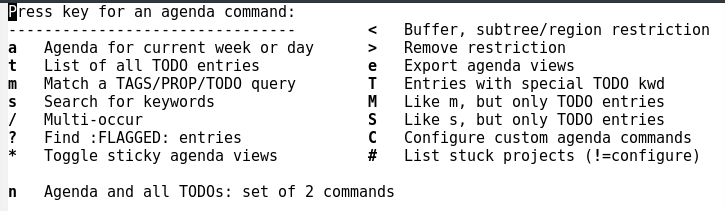
\includegraphics[width=0.9\textwidth]{org-agenda.png}
  \caption{Org agenda}
\end{figure}


\subsection{Commands in the Agenda Buffer}
\subsubsection{Motion}
\begin{description}
\item [n] next line
\item [p] previous line
\end{description}

\subsubsection{View/Go to Org File}
\begin{description}
\item [SPC] Display the original location of the item in another window.
\item [TAB] Go to the original location of the item in another window.
\item [RET] Go to the original location of the item and delete other windows.
\end{description}

\subsubsection{Change Display}
\begin{description}
\item [o] Delete other windows.
\item [v d or short d] Switch to day view.
\item [v w or short w] Switch to week view.
\item [f] Go forward in time to display the span following the current one. 
\item [b] Go backward in time to display earlier dates.
\item [.] Go to today.
\item [j] Prompt for a date and go there.
\item [v l or short l] Toggle Logbook mode.
\item [r]
\item [g] Recreate the agenda buffer.
\item [s] Save all Org buffers in the current Eamcs session, and also the location of IDs.
\end{description}

\subsubsection{Remote Editing}
\begin{description}
\item [0--9] Digit argument.
\item [t] Change to the TODO state of the item, both in the agenda and in the original Org file.
\item [C-k] Delete the current agenda item along with the entire subtree belonging to it in the original Org file. 
\item [C-c C-s] Schedule this item. With a prefix argument, remove the scheduling timestamp.
\item [C-c C-d] Set a deadline for this item. With a prefix argument, remove the deadline.
\item [S-$\rightarrow$] Change the timestamp associated with the current line by one day into the future.
\item [S-$\leftarrow$] Change the timestamp associated with the current line by one day into the past. 
\item [I] Start the clock on the current item.
\item [O] Stop the previously started clock.
\item [X] Cancel the currently running clock.
\item [J] Jump to the running clock in another window.
\end{description}

\subsubsection{Quit and Exit}
\begin{description}
\item [q] Quit agenda, remove the agenda buffer.
\item [x] Exit agenda, remove the agenda buffer and all buffers loaded by Emacs for the compilation of the agenda.
\end{description}
    

\subsection{Integration of Agenda and Calendar}
In order to include entries from the Emacs diary into Org mode's agenda, you only need to customize the variable
\lstset{language=Lisp}
\begin{lstlisting}
  (setq org-agenda-include-diary t)
\end{lstlisting}